\documentclass[pdftex,12pt,a4paper]{report}

\usepackage[portuguese,english]{babel}
\usepackage[T1]{fontenc} 
\usepackage[utf8]{inputenc}
\usepackage[pdftex]{graphicx}
\usepackage{minitoc}
\usepackage{hyperref}
\usepackage{indentfirst}
\usepackage[compact]{titlesec}
\usepackage{fancyhdr}
\usepackage{caption}
\usepackage{pgfplots}
\usepackage{pgfplotstable}
\usepackage{fixltx2e}
\usepackage{mathtools}
\usepackage{fancyhdr}
\usepackage{listings}
\usepackage{color}
\usepackage{sverb}
\usepackage[section]{placeins}

% JSON 

\colorlet{punct}{red!60!black}
\definecolor{background}{HTML}{EEEEEE}
\definecolor{delim}{RGB}{20,105,176}
\colorlet{numb}{magenta!60!black}

\lstdefinelanguage{json}{
    basicstyle=\normalfont\ttfamily,
    numbers=left,
    numberstyle=\scriptsize,
    stepnumber=1,
    numbersep=8pt,
    showstringspaces=false,
    breaklines=true,
    frame=lines,
    backgroundcolor=\color{background},
    literate=
     *{0}{{{\color{numb}0}}}{1}
      {1}{{{\color{numb}1}}}{1}
      {2}{{{\color{numb}2}}}{1}
      {3}{{{\color{numb}3}}}{1}
      {4}{{{\color{numb}4}}}{1}
      {5}{{{\color{numb}5}}}{1}
      {6}{{{\color{numb}6}}}{1}
      {7}{{{\color{numb}7}}}{1}
      {8}{{{\color{numb}8}}}{1}
      {9}{{{\color{numb}9}}}{1}
      {:}{{{\color{punct}{:}}}}{1}
      {,}{{{\color{punct}{,}}}}{1}
      {\{}{{{\color{delim}{\{}}}}{1}
      {\}}{{{\color{delim}{\}}}}}{1}
      {[}{{{\color{delim}{[}}}}{1}
      {]}{{{\color{delim}{]}}}}{1},
}

%Highlight
\newcommand{\shellcmd}[1]{\\\indent\indent\texttt{\footnotesize\# #1}\\}

\pagestyle{fancy}
\renewcommand*\thesection{\thechapter\arabic{section}}
\newcommand{\HRule}{\rule{\linewidth}{0.5mm}}
\begin{document}

\begin{titlepage}

\begin{center}


\includegraphics[width=0.15\textwidth]{./logo}\\[0.5cm]    

\textsc{\large Universidade de Aveiro \\[1cm]\large departamento de electrónica, telecomunicações e informática}\\[1cm]

\textsc{\large{47053}\large - Computação Visual \\[1cm]}

\HRule \\[0.5cm]
{ \huge \bfseries  Puzzle}\\[0.4cm]
{ \large \bfseries Implementação em WebGL de um Puzzle}\\[0.4cm]
\HRule \\[1cm]

\textsc{\small{8240 - MESTRADO INTEGRADO EM ENGENHARIA DE COMPUTADORES E TELEMÁTICA}}\\[1cm]

\begin{minipage}{0.4\textwidth}

\begin{flushleft} \large
\href{mailto:rafael.ferreira@ua.pt}{António Rafael da \\ Costa Ferreira }
 \small{\\NMec: 67405}
\end{flushleft}
\end{minipage}
\begin{minipage}{0.4\textwidth}

\begin{flushright} \large
\href{mailto:rodrigocunha@ua.pt}{Rodrigo Lopes \\ da Cunha}
\small{\\NMec: 67800}
\end{flushright}
\end{minipage}\\[1cm]

{\large Docente: Joaquim João Estrela Ribeiro Silvestre Madeira  }\\[0.5cm]

\vfill

{\large Dezembro de 2015 \\ 2015-2016}

\end{center}

\end{titlepage} %Titulo do Relatorio
\renewcommand{\headrulewidth}{0pt}

%Cabeçalhos de rodapé
\fancyhead{}
\fancyfoot{}
\lhead{Puzzle}
\rhead{CV - 2015/2016}
\lfoot{Rafael Ferreira nmec: 67405 \\ Rodrigo Cunha nmec: 67800}
\rfoot{\thepage}

%Renomear Comandos
\renewcommand*\contentsname{Conteúdos}
\renewcommand*\figurename{Figura}
\renewcommand*\tablename{Tabela}

%Conteúdos, dar paragrafo
\tableofcontents
%Headers
\renewcommand{\headrulewidth}{0.15pt}
\renewcommand{\thechapter}{}

\clearpage

\section{Introdução}
% o que, porquê e o objetivo
O trabalho proposto para o projeto da unidade curricular de Segurança é um IEDCS: Identity Enabled Distribution Control System. Para o  efeito foi necessário implementar uma Ebook Webstore, um WebService e um Player de reprodução dos Ebooks em formato de texto.

O objetivo deste sistema é garantir a máxima e possível segurança do serviço, utilizando os conhecimentos adquiridos na unidade curricular de Segurança. Para isso são necessários vários processos como por exemplo, a utilização de certificados HTTPS, a cifragem de todo o material existente, derivação de chaves e registo de utilizadores.	

O relatório reflete todos os passos e decisões tomadas na criação do sistema, assim como uma análise ao que foi mostrado na primeira apresentação e decisões que se tomaram depois desta, tecnologias utilizadas, descrição dos vários processos existentes e conclusão.

\clearpage

\section{JavaScript e WebGL}

\subsection{Arquitectura da implementação}

\begin{figure}[!htb]
\center
 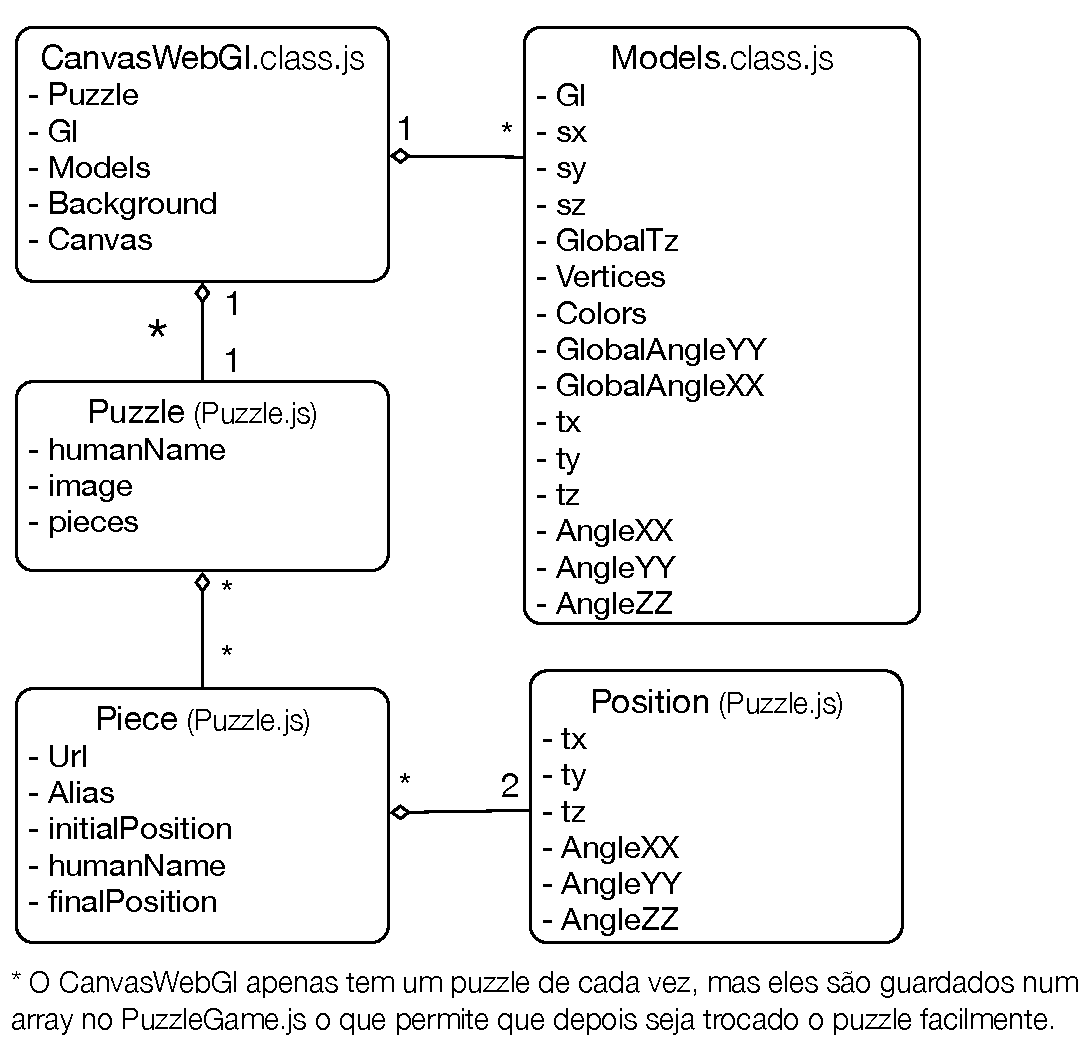
\includegraphics[width=70mm,scale=1]{classes.pdf}
 \caption{Diagrama da implementação desenvolvida}
 \label{fig:decifra_livro}
\end{figure}

Na implementação desenvolvida procurou-se uma solução que permitisse reutilizar o código e instanciar quantas peças e puzzles fosse preciso. Para isso criou-se uma class Models, que tem como atributos os que estão descritos em cima, que instância um modelo, independente dos outros que irá fazer uso das translações, rotações e outros métodos usados durante as aulas práticas. Para isso, esta class irá, no seu construtor instanciar uma única vez dois buffers, um chamado \textit{triangleVertexPositionBuffer} e outro  \textit{triangleVertexColorBuffer}, de resto, o \textit{initBuffers} é sempre chamado sempre que for feito um \textit{drawScene} para os arrays de buffers serem atualizados.

Já na class \textit{CanvasWebGl}, é onde o puzzle instância todos os modelos (peças), aplica as translações globais e independentes, é desenhada a cena, inicializado o modelo de fundo e inicializado o WebGl. 

Para alimentar a class \textit{CanvasWebGl}, foi criada uma class \textit{Puzzle} que tem todos os atributos necessários para instanciar um puzzle. O puzzle irá ter o seu \textit{humanName} que será apresentado ao utilizador, a \textit{image} que é a imagem final da solução do puzzle, e as \textit{pieces} que são as várias peças do puzzle.

A peça, terá o URL sendo este onde será obtido a lista de vértices e de cores para a peça. O alias é o usado para identificar a peça, tem de ser único para todas as peças existentes no Puzzle, o \textit{initialPosition} que identifica a posição inicial da peça e o \textit{finalPosition} que identifica a posição final da figura.

\subsection{JSON}

Para uma melhor definição de todos os puzzles usados no jogo foi criado um ficheiro JSON onde é possível criar todas as peças de cada puzzle e definir todos os atributos anteriormente detalhados. Este ficheiro é carregado inicialmente sempre que o jogo é iniciado, apresentando assim ao utilizador a lista de puzzles e inicializando o jogo com o puzzle inicial.

\begin{lstlisting}[language=json,firstnumber=1]
{
  "puzzles" : [
    {
      "humanName": "Level 1",
      "image" : "img/puzzles/puzzle1.png",
      "pieces" : [
        {
          "alias": "triangulo",
          "url": "modelos/trianguloBlue.txt",
          "humanName": "Triangulo Blue",
          "initialPosition" : {
            "tx": 0.2,
            "ty": 0.4,
            "tz": 0.5,
            "angleXX": 225,
            "angleYY": 45,
            "angleZZ": 45
          },
          "finalPosition" : {
            "tx": 0,
            "ty": 0,
            "tz": 0,
            "angleXX": 0,
            "angleYY": 0,
            "angleZZ": 0
          }
        }
      ]
    }
  ]
}
\end{lstlisting}

\subsection{JSON}


\end{document}